\documentclass{article}
\usepackage[landscape]{geometry}
\usepackage[american]{babel}
\usepackage{merriweather}
\pagestyle{empty}
\usepackage{graphicx}
\usepackage{makecell}
\usepackage{xcolor}
\usepackage{microtype}
\usepackage{hyperref}
  \hypersetup{colorlinks=true,allcolors=blue!40!black}
\begin{document}
\def\zoldversion{0.2.4}

\pagecolor{white}
\newcommand\slide[1]{%
  \pagebreak\topskip0pt\vspace*{\fill}%
  \begin{center}\Huge%
  #1
  \end{center}%
  \vspace*{\fill}%
}

\slide{
\includegraphics[scale=1]{../images/zerocracy-logo.pdf}\\
Zerocracy, Inc.\\[1em]
\large
Pitch Deck\\
\href{https://www.zerocracy.com}{www.zerocracy.com}}

\slide{Everybody thinks that robots will replace humans in their daily jobs, but we think something else will happen.}

\slide{With AI and modern communication platforms computers will manage people, not the other way around.}

\slide{Computers will plan and control our routine work, while we will do what we love to do---real work.}

\slide{Take software projects, where the problem is often management failure.}

\slide{That's because managers actually perform rather routine and boring tasks. We are just not good at it.}

\slide{AI actually can replace them, decreasing project failure rate.}

\slide{To our knowledge, AI technology has never played the role of an actual manager yet.}

\slide{This idea was born in Sep 2009.}

\slide{USPTO patent application was submitted in August 2011.\quad{\large US 12/703,202}}

\slide{The first three versions of the project management bot were deployed to production in 2010, 2013, and 2014.}

\slide{The current version \#4 was launched in March 2018 at \href{https://www.0crat.com}{0crat.com}.}

\slide{We have already processed transactions valued at over \$600K to date and managed
over 350 programmers who wrote over 700K lines of code for 48 projects and 17 clients.}

\slide{``After numerous failed attempts to bring projects to completion and
release them to our customers, I have finally found the method to solve my problems.
Zerocrat and the XDSD philosophy (especially microtasking) enable us to keep our
team focused on what is important instead of chasing down wild geese.''\\[1em]

\hfill\begin{tabular}{rl}
\makecell{%
%
\includegraphics[height=3em]{../images/yegor-bugayenko.jpg}
} &
\makecell[l]{%
---Michael Juliano\\
\Large SunSoft ERP Consulting\\[-8pt]
\Large Clearwater, Florida}
\end{tabular}}

\slide{We want to make this technology available for every software company in the world.}

\slide{Then, we want to expand our technology to other verticals, like construction, education, logistics, etc.}

\slide{We believe that computers must replace a traditional thousand-year-old management paradigm, which is not working anymore.}

\slide{%
\large%
\begin{tabular}{ccc}
  \makecell{
  
\includegraphics[height=10em]{../images/yegor-bugayenko.jpg}\\
  CEO and Founder\\
  \href{https://www.yegor256.com/about-me.html}{Yegor Bugayenko}\\
  \normalsize Author of ``Elegant Objects'' book\\
  \normalsize PMP, SCEA, PRINCE2, RUP}
&
  \makecell{%
  
\includegraphics[height=10em]{../images/kiril-cherniavsky.jpg}\\
  Lead Architect\\
  \href{https://github.com/g4s8}{Kiril Cherniavsky}\\
  \normalsize Open source activist,\\
  \normalsize Co-architect of EO Language}
&
  \makecell{%
  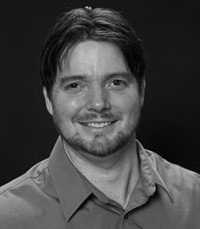
\includegraphics[height=10em]{../images/erik-larson.jpg}\\
  Advisor\\
  \href{https://www.linkedin.com/in/erik-larson-b287ba9/}{Erik J. Larson}, PhD\\
  \normalsize NLP/AI expert\\
  \normalsize DARPA-funded AI startup founder}
\end{tabular}\\[2em]
\begin{tabular}{ccc}%
  \makecell{%
  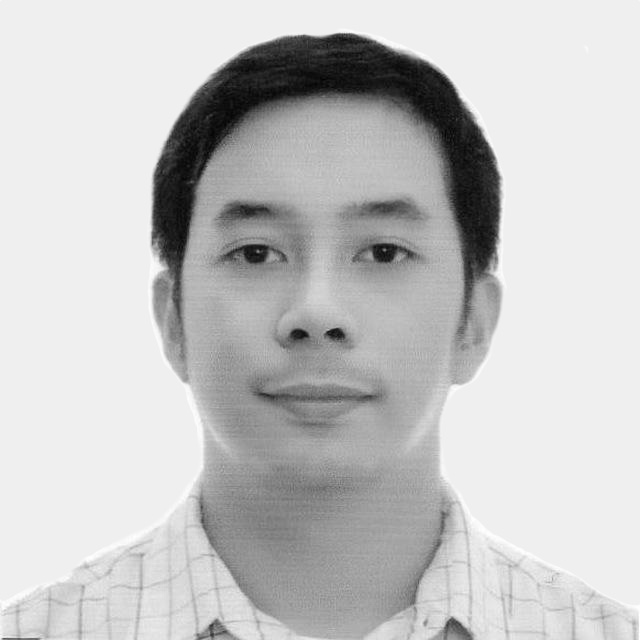
\includegraphics[height=10em]{../images/carlos-miranda.jpg}\\
  Senior Developer\\
  \href{https://github.com/carlosmiranda}{Carlos Miranda}\\
  \normalsize Certified Java Programmer\\
  \normalsize Remote Teams Advocate}
&
  \makecell{%
  
\includegraphics[height=10em]{../images/krzysztof-krason.jpg}\\
  Senior Developer\\
  \href{https://github.com/krzyk}{Krzysztof Kraso\'n}\\
  \normalsize SCJP, Open Source Enthusiast\\
  \normalsize Qulice architect}
&
  \makecell{%
  
\includegraphics[height=10em]{../images/george-aristy.jpg}\\
  Senior Developer\\
  \href{https://github.com/llorllale}{George Aristy}\\
  \normalsize Java Certified Programmer\\
  \normalsize Zold Co-architect}
\end{tabular}%
}

\slide{%
  \Large
    \href{https://twitter.com/0crat}{Twitter}
    \quad
    \href{https://facebook.com/zerocracy}{Facebook}
    \quad
    \href{https://www.zerocracy.com/blog.html}{Blog}
  \\[1em]
  \Large
    \href{https://papers.zold.io/freelance-deck.pdf}{Freelance Deck}
    \quad
    \href{https://papers.zold.io/executive-summary.pdf}{Executive Summary}
  \\[1em]
  \Large
    555 Bryant Str, Ste 470\\
    Palo Alto, CA 94301\\
    408.692.4742\\
    \href{mailto:team@zerocracy.com}{team@zerocracy.com}
  \\[1em]
  \normalsize\texttt{\zoldversion\qquad\today}
}

\end{document}
